\documentclass{article}
\usepackage[spanish]{babel}
\usepackage{url}
\author{Claude E. Shannon}
\title{Una teor\'{\i}a matem\'{a}tica de la comunicaci\'{o}n}
\date{1948}
\begin{document}
\maketitle

\begin{abstract}
  Esta es una traducci\'{o}n al espa\~{n}ol del art\'{\i}culo
  publicado por Shannon en {\em The Bell System Technical Journal},
  realizado a base del PDF disponible en
  \url{http://cm.bell-labs.com/cm/ms/what/shannonday/shannon1948.pdf}
  como un esfuerzo colectivo de estudiantes de octavo semestre del ITS
  de la FIME de la UANL por puntos extra en la unidad de aprendizaje
  {\em Teor\'{\i}a de la informaci\'{o}n y m\'{e}todos de
    codificaci\'{o}n}, impartida por Dra.\ Elisa Schaeffer en la
  primavera del 2013.
\end{abstract}

\documentclass{article}
\title{Cartesian closed categories and the price of eggs}
\author{Jane Doe}
\date{September 1994}
\begin{document}
   \maketitle
   Hello world!
\end{document}
 % pp. 1--6
4. Representacion grafica de procesos Markovianos

Los procesos estocasticos del tipo descrito arriba son matematicamente conocidos como Procesos Markovianos Discretos y han sido estudiados extensivamente en la literatura.^{6} El caso general puede ser descrito de la siguiente manera: Existe un numero finito de posibles "estados" de un sistema; S_{1}, S_{2}, ...,S_{n}. Adem\'{a}s existen un conjunto de probabilidades de transicion; p_{i}(j) la probabilidad que si el sistema esta en estado S_{i} entonces enseguida vaya al estado S_{j}. Para realizar este proceso Markoviano en una fuente de información solo necesitamos asumir que una letra es producida para cada transicion desde un estado a otro. Los estados corresponderán al ``residuo de influencia'' de letras precedentes. \\
La situacion puede ser representada graficamente como se muestra en las figuras 3, 4 y 5. Los "estados" son los puntos de union

% aqui va figura 3

en la grafica y las probabilidades y letras son producidas para una transicion son dadas ademas de la linea correspondiente. La figura 3 es para el ejemplo B en la seccion 2, mientras que la figura 4 corresponde al ejemplo C. En la figura 3

%figura 4

solamente hay un estado ya que letras sucesivas son independientes. En la figura 4 hay tantos estados como letras. \newline
Si un ejemplo de un triagrama fuera construido, habr\'{i}a por maximo n^{2} estados correspondiendo a los posibles pares de letras precediendo a uno que haya sido elegido. La figura 5 es un grafo para el caso de estructura de palabras en el ejemplo D. Aqui S corresponde a el simbolo ``espacio''. \newline

5. Fuentes erg\'{o}dicas y mixtas.

Como se ha indicado anteriormente, una fuente discreta para nuestros propositos puede ser considerada representada por un proceso Markoviano. Entre los posibles procesos discretos Markovianos existe un grupo con propiedades especiales con importancia en la teoria de la comunicacion. Esta clase especial consiste en los procesos ``ergodicos'' y deberiamos de llamar a las fuentes correspondientes, fuentes ergodicas. Aunque una definicion rigurosa de los procesos ergodicos es algo complicada, la idea general es simple. En un proceso ergodico cada secuencia producida por el proceso permanece igual en sus propiedades estadisticas. Por lo tanto las frecuencias de letras, las frecuencias de bigramas, etc., obtenidos de una secuencia en particulas, se acercaran a un limite definido conforme la longitud de las secuencua aumenta, independientemente de la secuencia en particular. En realidad esto no es meramente cierto para cada secuencia pero el grupo para el cual esto es falso tiene una probabilidad de cero. Practicamente, la propiedad ergodica significa homogeneidad estadistica. \\
Todos los ejemplos de lenguaje artificial dados anteriormente son ergodicos. Esta propiedad está relacionada a la estructura de los grafos correspondientes. Si el grafo tiene las siguientes dos propiedades el proceso correspondiente será ergodico:

\begin{enumerate}
   \item El grafo no consiste de dos partes aisladas A y B dado que es imposible ir desde los puntos de union en la parte A a los puntos de union en la parte B a traves de las lineas del grafo en la direccion de las flechas y tambien es imposible ir desde las uniones en la parte B a las uniones en la parte A. 
   \item 
\end{enumerate}

\begin{equation}
b = a - 2
\end{equation}
 % pp. 7--18
Este doble proceso puede decodificar el mensaje original en los mismo s\'{i}mbolos, pero con un radio de compresi\'{o}n promedio de $\frac{7}{8}$.

Como un segundo ejemplo considere una fuente que produce una secuencia de A's y B's con probabilidad p para A y q por B. Si p << q tenemos que

\begin{equation}
H = - log p^p (1 - p)^1^-^p
= -p log p(1-p)^(^1^-^p^)^/^p
= p log \frac{e}{p}
\end{equation}

En tal caso uno puede construir una codificaci\'{o}n del mensaje sobre un canal de 0, 1 lo suficientemente buena mediante el env\'{i}o de una secuencia especial, por ejemplo 0000, para el s\'{i}mbolo poco frecuente A y a continuaci\'{o}n, una secuencia indicando el n\'{u}mero siguiente de B's. Esto podr\'{i}a ser indicado por una representaci\'{o}n binaria con todos los n\'{u}meros que contienen la secuencia especial eliminada. Todos los n\'{u}meros hasta el 16 son representados como de costumbre; el 16 es representado por el siguiente n\'{u}mero binario despues de 16 que no contiene 4 ceros, es decir, 17  = 10001, etc.

Se puede demostrar que a medida que $p\rightarrow{0}$ los enfoques de codificaci\'{o}n ideales proporcionan la longitud de la secuencia especial es ajustada correctamente.

\part{El canal discreto con ruido}
\label{part:2}

\chapter{Representaci\'{o}n de un canal discreto con ruido}
\label{sec:11}

Ahora consideremos el caso en donde la señal es perturbada por ruido durante la transmisi\'{o} o en algunas de las terminales. Esto significa que la señal recibida no es necesariamente el mismo que el enviado por el transmisor. Dos casos pueden ser distinguidos. Si una señal particular transmitida siempre produce la misma señal recibida, es decir, la señar recibida es una funcion definida de la señal transmitida, entonces el efecto puede ser llamado distorsi\'{o}n. Si la función tiene inversa -las dos señales transmitidas no deben de producir la misma señal recibida- la distorsi\'{o} puede ser corregida, al menos al principio, solamente por la realizaci\'{o}n de la operaci\'{o}n de la funci\'{o}n inversa de la señal recibida.

El caso de inter\'{e}s aqu\'{i} es aquel en el que la señal no siempre se someta al mismo cambio en la transmisi\'{o}n. En este caso podemos asumir que la señal recibida E es una funci\'{o} de la señal de transmisi\'{o}n S y una segunda variable, el ruido N.

\begin{equation}
E = f\left (S,\right N)
\end{equation}

El ruido es considerado como una variable de probabilidad igual al mensaje que estaba por encima. En general, esto puede ser representado como un proceso estoc\'{a}stico adecuado. El tipo m\'{a}s general de canales discretos con ruido que consideramos es una generalizaci\'{o}n de el canal libre de ruido de estado finito descrito anteriormente. Podemos asumir un n\'{u}mero finito de estados y un conjunto de probabilidades

\begin{equation}
P_{\alpha, i}\left ( \beta , \right j).
\end{equation}

Esta es la probabilidad, si el canal est\'{a} en el estado $\alpha$ y el s\'{i}mbolo $i$ es transmitido, el s\'{i}mbolo $j$ sera recibido y el canal se queda en estado $\beta$. As\'{i} $\alpha$ y el rango de $\beta$ sobre las posibles señales recibidas. En el caso de que los s\'{i}mbolos sucesivos son perturbados de forma independiente por el ruido solo hay un estado, y el canal es descrito por el conjunto de probablidades de transici\'{o}n $P_{i}\left (j\right)$, la probabilidad de transmitir un s\'{i}mbolo $i$ sera recibido como $j$·

Si el canal con ruido es alimentado por una fuente hay dos procesos en trabajo: la fuente y el ruido. Por lo tanto hay un n\'{u}mero de entrop\'{i}as que se pueden calcular. En primer lugar est\'{a} la entrop\'{i}a $H(x)$ de la fuente o de la entrada al canal (\'{e}stos ser\'{a}n iguales si el transmisor es no singular). La entrop\'{i}a de la salidad del canal, es decir, la señal recibida se denota por $H(y)$. En el caso sin ruido $H(y) = H(x)$. El conjunto de entrop\'{i}as de entrada y salida ser\'{a} $H\left(x\right y)$. Finalmente donde haya dos entrop\'{i}as condicionales $H_{x}(y)$ y $H_{y}(x)$, la entrop\'{i}a de la salida cuando la entrada es conocida y a la inversa. Entre esas cantidades tenemos las relaciones

\begin{equation}
H\left (x,\right y) = H(x) + H_{x}(y) = H(y) + H_{y}(x).
\end{equation}

Todas estas entrop\'{i}as se pueden medir en funci\'{o}n de por segundo o en funci\'{o}n de cada s\'{i}mbolo.

\clearpage

\chapter{Equivocaci\'{o}n y capacidad de canal}
\label{sec:12}

Si el canal es con ruido por lo general no es posible el reconstruir el mensaje original o la señal transmitida con certeza por cualquier operaci\'{o} efectuada sobre la señal recibida $E$. Hay, sin embargo, maneras de transmitir la informaci\'{o}n que son \'{o}ptimas en el combate contra el ruido. Este es el problema que consideramos ahora

Supongamos que hay dos posibles s\'{i}mbolos 0 y 1, y estamos transmitiendo a una velocidad de 1000 s\'{i}mbolos por segundo con probabilidad de $p_{0} = p_{1} = \frac{1}{2}$. Por lo tanto nuestra fuenta est\'{a} produciendo informaci\'{o}n a la velocidad de 1000 bits por segundo. Durante la transmisi\'{o}n del ruido se introduce errores de manera que, en promedio, 1 en 100 se recibieron incorrectamente (un 0 como 1, o 1 como 0). ¿Cu\'{a}l es la tasa de transmisi\'{o}n de informaci\'{o}n? Ciertamenet menos de 1000 bits por segundo aproximadamente el 1\% de los s\'{i}mbolos recibidos son correctos. Nuesto primer impulso podr\'{i}a decir que la tasa es de 990 bits por segundo, simplemente el n\'{u}mero de errores esperados. Esto no es satisfactorio ya que no se tiene en cuenta la falta de conocimiento de d\'{o}nde se producen los errores del destinatario. Es posible llevarlo a un caso extremo y supongamos que el ruido es tan grande que los s\'{i}mbolos recibidos son totalmente independientes de los s\'{i}mbolos transmitidos. La probalidad de recibir $1$ es $\frac{1}{2}$ en todo lo que se transmite y de manera similar para 0. Luego, alrededor de la mitada de los s\'{i}mbolos recibidos son correctos debido al azar, y nos estar\'{i} dando el cr\'{e}dito del sistema para la transmisi\'{o}n de 500 bits por segundo, cuando en realidad la informaci\'{o} no se transmite en absoluto. Igualmente la transmisi\'{o}n "correcta" se obtendr\'{i}a mediante la dispensaci\'{o}n con el canal entero y lanzando una moneda en el punto de recepci\'{o}n.

FALTA

\begin{theorem}
\label{th:10}
Si el canal de correcci\'{o}n...
\end{theorem}

FALTA

\begin{figure}[!ht]
\centerline{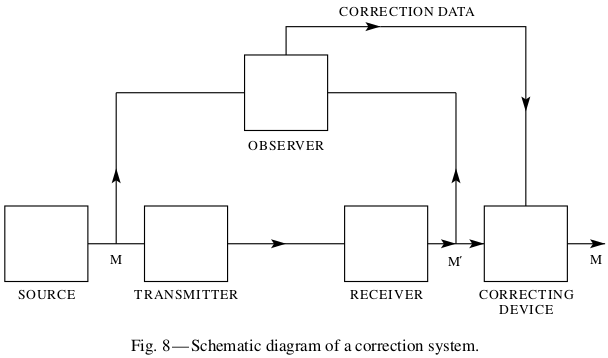
\includegraphics[width=120mm]{Imagenes/Pagina21-Figura8.png}}
\caption{Un diagrama esquem\'{a}tico de un sistema de correcci\'{o}n.}
\label{fig:8}
\end{figure}

FALTA

\begin{exmp}
Suponga que los errores suceden al azar...
\end{exmp}

FALTA

\begin{theorem}
\label{th:11}
Que un canal discreto tenga
\end{theorem}

FALTA

\clearpage

\chapter{El teorema fundamental para un canal discreto con ruido}
\label{sec:13}

\begin{figure}[!ht]
\centerline{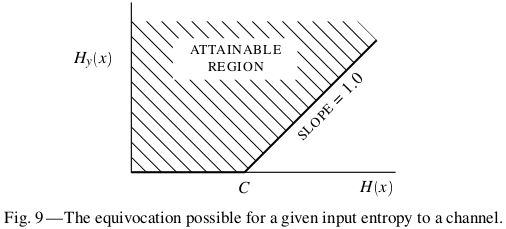
\includegraphics[width=100mm]{Imagenes/Pagina22-Figura9.png}}
\caption{La equivocaci\'{o}n posible para una entropia de entrada dada
  a un canal.}
\label{fig:9}
\end{figure}

FALTA

\begin{figure}[!ht]
\centerline{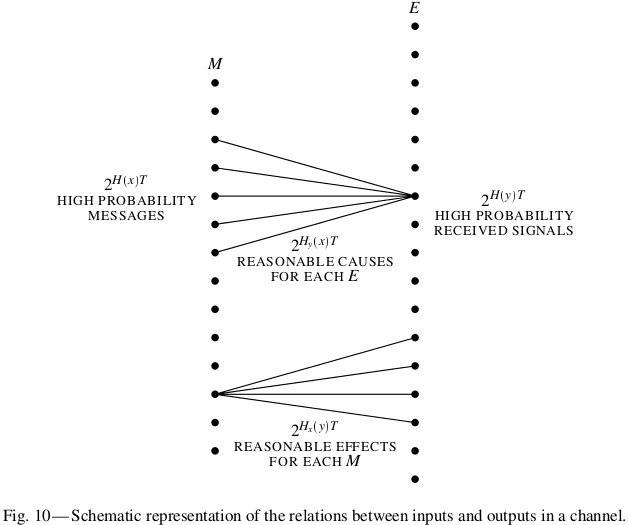
\includegraphics[width=140mm]{Imagenes/Pagina23-Figura10.png}}
\caption{Una representaci\'{o}n esquem\'{a}tica de las relaciones
  entre las entradas y salidas en un canal.}
\label{fig:10}
\end{figure}

FALTA

\clearpage

\chapter{Discussion}
\label{sec:14}

FALTA

 % pp. 19--31
Hola

\begin{equation}
a = b + 2
\end{equation}
 % pp. 32--35
{\textexclamdown}Hola, mundo!

\section{Entrop\'ia de la suma de dos conjuntos}

	Si tenemos dos conjuntos de funciones $f_{\alpha}(t)$ y
	$g_{\beta}(t)$ podemos formar un nuevo conjunto por
	``adici\'on''. Supongamos que el primer conjunto tiene la
	funci\'on de densidad de probabilidad $p(x_{1},...,x_{n})$ y
	el segundo $q(x_{1},...,x_{n})$.  Despu\'es la funci\'on de
	densidad para la adici\'on es dada por la convoluci\'on
	
	\begin{equation} r(x_{1},...,x_{n}) = \int \cdots \int
		p(y_{1},...,y{n})q(x_{1}-y_{1},...,x_{n}-y_{n}) \diff y_{1}... \diff y_{n} \end{equation}
	
	F\'isicamente esto corresponde a sumar los ruidos o se\~nales
	representados por los conjuntos originales de las funciones
	
		
	El siguiente resultado es derivado en el Ap\'endice 6
	
    \begin{theorem} Deje que la potencia media de los 2 conjuntos sea
    $N_{1}$ y $N_{2}$ y deje que sus poderes de entrop\'ia sean
    $\bar{N}_1$ y $\bar{N}_2$ . Entonces, el poder de entrop\'ia de
    la suma, $N_{3}$, est\'a delimitado
    por \begin{equation} \bar{N}_1+\bar{N}_2 \le \bar{N}_3 \le
    N_{1}+N_{2}.  \end{equation} \end{theorem}
	
	El ruido blanco Gaussiano tiene la peculiar propiedad que
	puede absorber cualquier otro ruido o conjunto de se\~nales
	que puede ser a\~nadido a la misma con una potencia de
	entrop\'ia resultante aproxim\'adamente igual a la suma de a
	potencia ruido blanco y la potencia de la se\~nal (medida
	apartir del valor promedio de la se\~nal, que es normalmente
	cero), siempre que la potencia de la se\~{n}al es peque\~na,
	en cierto sentido, en comparaci\'on con el ruido.
	
	Considere el espacio de la funci\'on asociada con estos
	conjuntos que tienen dimensiones n. El ruido blanco
	corresponde a la distribuci\'on Gaussiana esf\'erica en este
	espacio. El conjunto de la se\~nal corresponde a otra
	distribuci\'on de probabilidad, no necesariamente Gaussiana o
	esf\'erica. Deje que los segundos momentos de esta
	distribuci\'on alrededor de su centro de gravedad sea
	$a_{ij}$.  Es decir, si p($x_{1},...,x_{n}$) es la funci\'on
	de distribuci\'on de densidad \begin{equation}
	a_{ij}=\int \cdots \int
	p(x_{i}-\alpha_{i})(x_{j}-\alpha_{j}dx_{1} \cdots
	dx_{n}) \end{equation} donde $\alpha_{i}$ son las coordenadas
	del centro de gravedad. Ahora $a_{ij}$ es una forma
	cuadr\'atica positiva, y podemos rotar nuestro sistema de
	coordenadas para alinearla con las direcciones principales de
	esta forma. $a_{ij}$ es entonces reducido a la forma diagonal
	$b_{ii}$. Se requiere que cada $b{ii}$ sea peque\~no comparado
	con N, el cuadrado del radio de la distribuci\'on esf\'erica.
	
	En este caso, la convoluci\'on del ruido y se\~nal producen
	aproximadamente una distribuci\'on Gaussiana cuya forma
	cuadr\'atica correspondiente es \begin{equation} N +
	b_{ii}.  \end{equation}
	
	El potencial de entrop\'ia de esta distribuci\'on
	es \begin{equation} [\Pi(N +
	b_{ii})]^\frac{1}{n} \end{equation} o
	aproximadamente \begin{equation} = [(N)^n + \Sigma
	b_{ii}(N)^n-1]^\frac{1}{n} \end{equation} \begin{equation} = N
	+ \frac{1}{n}\Sigma b_{ii}.  \end{equation} El \'ultimo
	t\'ermino es la potencia de la se\~nal, mientras que el
	primero es la potencia del ruido.
	
	
	\chapter{El canal continuo}
	
\section{La capacidad de un canal continuo}	
	
	En un canal continuo de las se\~nales de entrada o
	transmitidas ser\'an funciones continuas de tiempo $f(t)$
	pertenecientes a un determinado conjunto, y la señales de
	salida o recibidas ser\'an versiones perturbadas de
	estas. Vamos a considerar solo el caso en que ambas se\~nales
	transmitidas y recibidas se limitan a una determinada banda
	$W$. Pueden ser despu\'es identificadas por un tiempo $T$, por
	los n\'umeros $2TW$, y su estructura estad\'istica de las
	funciones de distribuci\'on finitos tridimensionales. As\'i
	las estad\'isticas de la se\~nal transmitida ser\'a
	determinada por
	\begin{equation}
		P(x_{1}, \cdots ,x_{n}) = P(x)
	\end{equation}	 
	y los del ruido por la distribuci\'on de probabilidad condicional
	\begin{equation}
		P_{x1, \cdots ,xn} (y_{1}, \cdots ,y_{n}) = P_{x}(y).
	\end{equation}
	
	La tasa de transmisi\'on de informaci\'on por un canal
	continuo se define de una manera an\'aloga a la de un canal
	separado, esto es \begin{equation} R =
	H(x)-H_{y}(x), \end{equation} donde $H(x)$ es la entrop\'ia de
	la entrada y $H_{y}(x)$ el equ\'ivoco. La capacidad del canal
	$C$ se define como el m\'aximo de R cuando var\'ian la entrada
	para todos los conjuntos posibles. Esto significa que en una
	aproximaci\'on dimensional finita debemos variar $P(x) =
	P(x_{1},...,x_{n})$ y maximizar \begin{equation} - \int
	P(x) \log P(x)dx + \int\int
	P(x,y)\log \frac{P(x,y)}{P(y)}dx \diff y.  \end{equation} Esto puede
	ser escrito \begin{equation} \int\int
	P(x,y) \log \frac{P(x,y)}{P(x)P(y)}dx \diff y \end{equation} usando
	el hecho que $\int\int P(x,y)\log P(x)dx \diff y = \int P(x)\log
	P(x)dx$. La capacidad del canal se expresa as\'i:
	\begin{equation}
		C = \limsup_{T\to \infty P(x)} \frac{1}{T}\int\int P(x,y)\log \frac{P(x,y)}{P(x)~
		P(y)}dx \diff y.
	\end{equation}
	
	Es obvio que en esta forma $R$ y $C$ son independientes del
	sistema de coordenadas dado que el numerador y denominador en
	$\log\frac{P(x,y)}{P(x)P(y)}$ ser\'a multiplicado por los
	mismos factores cuando $x$ y $y$ son transformados en
	cualquier forma uno a uno. Esta expresi\'on integral para $C$
	es m\'{a}s general que $H(x)-H_{y}(x)$. Correctamente
	interpretada (ver Anexo 7) que siempre existir\'a mientras
	$H(x)-H_{y}(x)$ puede asumir una forma indeterminada $\infty
	- \infty$ en algunos casos. Esto ocurre, por ejemplo, si $x$
	est\'a limitada a una superficie de menos dimensiones que $n$
	en su aproximaci\'on $n$ dimensional.
	
	Si la base logar\'itmica utilizada en computaci\'on $H(x)$ y
	$H_{y}(x)$ es dos entonces $C$ es el n\'umero m\'aximo de
	d\'igitos binarios que pueden ser enviados por segundo a
	trav\'es del canal con equivocaci\'on arbitrariamente
	peque\~na, al igual que en el caso discreto. Esto se puede ver
	f\'isicamente al dividir el espacio de se\~nales en un gran
	n\'umero de celdas peque\~nas y suficientemente peque\~no para
	que la densidad de probabilidad $P_{x}(y)$ de la se\~nal x que
	est\'{a}q siendo perturbado hasta el punto de que $y$ es
	sustancialmente constante en una celda (ya sea de $x$ o
	$y$). Si las celdas son consideradas como puntos distintos, la
	situaci\'on es esencialmente la misma que un canal discreto y
	las pruebas usadas se aplicar\'an all\'{a}. Pero est\'{a}
	claro que f\'isicamente esta cuantificaci\'on del volumen en
	puntos individuales no puede de ninguna manera pr\'actica
	alterar significativamente la respuesta final, siempre que las
	regiones sean suficientemente peque\~nas. As\'i la capacidad
	ser\'{a} el l\'imite de las capacidades de las subdivisiones
	discretas y esto es es s\'olo la capacidad continua definida
	anteriormente.
	
	En el lado matem\'atico se pede demostrar primero (ver el
	Ap\'endice 7) que si $u$ es el mensaje, $x$ es la se\~nal, $y$
	es la se\~nal recibida (perturbada por el ruido) y $v$ es el
	mensaje recuperado, entonces
	\begin{equation}
		H(x) - H_{y}(x) \le H(u) - H_{v}(u).
	\end{equation}	 
	
	Independientemente de lo que las operaciones realizan en $u$
	para obtener $x$ o en $y$ para obtener $v$. No importa como
	modificamos los d\'igitos binarios para obtener la se\~nal, o
	como decodificamos la se\~nal recibida para recuperar el
	mensaje, la tasa discreta para los d\'igitos binarios no
	excede la capacidad del canal que tenemos definida. Por otra
	parte, es posible bajo condiciones muy generales encontrar un
	sistema de codificaci\'on para transmitir d\'igitos binarios
	en la tasa $C$ con peque\~na equivocaci\'on o frecuencia de
	errores como se desee. Este es el caso, por ejemplo, si,
	cuando tomamos un espacio finito de aproximaci\'on para las
	funciones de las se\~nales, $P(x,y)$ es continuo tanto en $x$
	como en $y$, excepto en un conjunto de puntos de probabilidad
	cero.
	
	Un caso especial se produce cuando el ruido se a\~nade a la
	se\~nal y es independiente de ello (en el sentido de la
	probabilidad). Entonces $P_{x}(y)$ es una funci\'on s\'olo de
	la diferencia $n = (y-x)$,
	\begin{equation}
		P_{x}(y) = Q(y-x).
	\end{equation}
	
	%%%%%%%%%%%%% PAGINA 43 ES LA SIGUIENTE %%%%%%%%%%	
	
	y nosotros podemos asignar una entrop\'ia definida al ruido (independientemente de 
	las estad\'isticas de la se\~nal), es decir, la entrop\'ia de la distribuci\'on
	$Q(n)$. Esta entrop\'ia se denotar\'a por $H(n)$.
	
	\begin{em}
		Teorema 16: Si la se\~nal y el ruido son independientes y la se\~nal recibida
		es la suma de se\~nal transmitida y el ruido entonces la tasa de transmisi\'on es
	\end{em}
	
	\begin{equation}
		R = H(y) - H(n),
	\end{equation}
	
	es decir, la entrop\'ia de la se\~nal recibida menos la entrop\'ia del ruido. La
	capacidad del canal es
	
	\begin{equation}
		C = \limsup_{P(x)} H(y) - H(n)
	\end{equation}
	
	Tenemos, desde $y = x+n$
	
	\begin{equation}
		H(x,y) = H(x,n).
	\end{equation}
	
	Expandiendo el lado izquierdo y utilizando el hecho de que $x$ y $n$ son independientes
	
	\begin{equation}
		H(y) + H_{y}(x) = H(x) + H(n).
	\end{equation}
	
	Por lo tanto
	
	\begin{equation}
		R = H(x) - H_{y}(x) = H(y) - H(n).
	\end{equation}
	
	Puesto que $H(n)$ es independiente de $P(x)$, maximizando R requiere maximizar $H(y)$,
	la entrop\'ia de la se\~nal recibida. Si existen ciertas restricciones en el conjunto
	de las se\~nales transmitidas, la entrop\'ia de la se\~nal recibida debe ser maximizada
	sujeto a esas restricciones.
	
	\bigskip
	25. CAPACIDAD DE LA SE\~NAL  CON UNA LIMITACI\'ON DE POTENCIA MEDIA
	\bigskip	
	
	Una sencilla aplicaci\'on del teorema 16 es el caso cuando el ruido es un ruido
	t\'ermico blanco y las se\~nales transmitidas est\'an limitadas a un cierto 
	promedio de potencia $P$. Luego las se\~nales recibidas tienen una potencia media
	$P + N$ donde $N$ es la potencia media del ruido. La entrop\'ia m\'axima para las
	se\~nales recibidas se produce cuando tambi\'en forman un ruido blanco ya que 
	es la entrop\'ia mayor posible para una potencia $P + N$ y puede obtenerse mediante
	una elecci\'on adecuada de las se\~nales transmitidas, a saber, si forman un conjunto
	de ruido blanco de potencia $P$. La entrop\'ia (por segundo) del conjunto recibido es luego
	
	\begin{equation}
		H(y) = W\log 2\pi e(P+N),
	\end{equation}
	
	Y la entrop\'ia de ruido es
	
	\begin{equation}
		H(n) = W\log 2\pi eN.
	\end{equation}
	
	La capacidad del canal es
	
	\begin{equation}
		C = H(y) - H(n) = W\log \frac{P + N}{N}.
	\end{equation}
	
	Resumiendo tenemos lo siguiente:
	
	Teorema 17: La capacidad de un canal de banda $W$ de potencia perturbada por el ruido
	t\'ermico blanco $N$ cuando la potencia de transmisi\'on media se limita a $P$ viene
	dada por
	
	\begin{equation}
		C = W\log \frac{P + N}{N}.
	\end{equation}
	
	Esto significa que por sistemas de codificaci\'on suficientemente implicados se puede
	transmitir d\'igitos binarios a la tasa $W \log_{2}\frac{P + N}{N}$ bits por segundo,
	con arbitrariamente peque\~na frecuencia de errores. No es posible transmitir a una
	velocidad mayor por cualquier sistema de codificaci\'on sin una frecuencia
	definida positiva de errores.
	
	Para aproximar esta limitaci\'on de la tasa de transmisi\'on, las se\~nales transmitidas
	deben aproximarse, en propiedades estad\'isticas, un ruido blanco. Un sistema que se 
	aproxima a la tasa ideal puede ser descrito como sigue: Sea $M = 2^s$
	
	%%%%%%%%%%%%%% SIGUE LA PAGINA 44
	Meh meh
	
	%Ecuacion sin numero
	\begin{displaymath}
		x^{2}+y^{2}=h^2
	\end{displaymath}

	%Ecuacion
	\begin{equation}
		p\left ( x_{1},...,x_{n}\right )
	\end{equation}

	%Ecuacion
	\begin{equation}
		{H}'=-\lim_{n\rightarrow \infty }\frac{1}{n}\int \cdots \int p\left ( 							x_{1},...,x_{n}\right ) \log p\left ( x_{1},...,x_{n}\right ) \diff x_{1}... \diff x_{n}
	\end{equation}

	%Ecuacion
	\begin{equation}
		{H}'=\log \sqrt{2\pi eN}
		\newline
		H=W\log 2\pi eN
	\end{equation}		
	



 % pp. 41--47


\end{document}
